\documentclass[a4paper, 12pt, one column, aas_macros]{article}

%% Language and font encodings. This says how to do hyphenation on end of lines.
\usepackage[english]{babel}
\usepackage[utf8x]{inputenc}
\usepackage[T1]{fontenc}
\usepackage{aas_macros}

%% Adds in official euro sign
\usepackage[official]{eurosym}

%% Sets page size and margins. You can edit this to your liking
\usepackage[top=1.3cm, bottom=2.0cm, outer=2.5cm, inner=2.5cm, heightrounded,
marginparwidth=1.5cm, marginparsep=0.4cm, margin=2.5cm]{geometry}

%% Useful packages
\usepackage{graphicx} %allows you to use jpg or png images. PDF is still recommended
\graphicspath{ {./images/} } % Sets base path for images
\usepackage[colorlinks=False]{hyperref} % add links inside PDF files
\usepackage{amsmath}  % Math fonts
\usepackage{amsfonts} % More fonts
\usepackage{amssymb}  % Symbols
\usepackage{subcaption} % Sub-figure captions
\usepackage{listings}   % Code style text

%% Citation package
\usepackage[nottoc]{tocbibind} %% Add refs to ToC
\usepackage[square,numbers]{natbib}
\bibliographystyle{dinat}
% \setcitestyle{authoryear,open={(},close={)}}

%% Change content and figure titles
\renewcommand{\contentsname}{Contents}
\renewcommand{\figurename}{Figure}

\def\code#1{\texttt{#1}}

%% Begin document
\begin{document}

%% Create title page
\begin{titlepage}
    \title{
        SFS | Clean install and running setup
    }
    \author{PowerMonitoring 2020}
    \date{\today}
    \thispagestyle{empty}
\end{titlepage}

\maketitle
\thispagestyle{empty}

\newpage
\thispagestyle{empty}
\tableofcontents
\newpage
\setcounter{page}{1}
\section{Logger}
\section{Setup}
To continue where this project has left of, internet is definitely required. We use a hotspot to do everything that required an internet connection.\newline
The cluster also needs to be setup correctly. Make sure all the power connectors from the black PCB's are connected to the correct Raspberry Pi's. We labelled the Pi's from bottom to top: 0 - 3, with the highest up one being the "g" pi, or Grafana pi. In our setup we conected them to the PCB as follows:
\begin{table}[h]
\centering
\begin{tabular}{|l|l|}
\hline
Address & Pi \\ \hline
0x40 & 0 \\ \hline
0x41 & 1 \\ \hline
0x42 & 2 \\ \hline
0x43 & 3 \\ \hline
0x44 & G \\ \hline
\end{tabular}
\end{table}
\newline
With the addresses being on the following places:
\begin{figure}[h]
	\centering
	\begin{subfigure}[b]{0.4\linewidth}
    		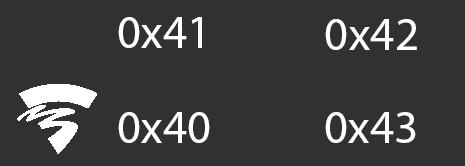
\includegraphics[width=\linewidth]{pcb-ina-0.png}
    		\caption{Bottom PCB}
    	\end{subfigure}
    \begin{subfigure}[b]{0.4\linewidth}
    		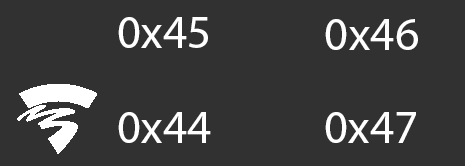
\includegraphics[width=\linewidth]{pcb-ina-1.png}
    		\caption{Top PCB}
    \end{subfigure}
    \caption{PCB INA connector layout, following page 18 of \url{http://www.ti.com/lit/ds/symlink/ina260.pdf}}
    \label{inapcb}
\end{figure}\newline
After that, make sure every Pi has it's own ethernet connection to the switch. If everything is setup correctly, it should work with the provided settings file "pis.xml" in the ina260 folder, the file will be required when starting the logger.\newline
\newline
\textbf{NOTE:}
\begin{itemize}
	\item In the current release of Debian Buster, the Pi picks only one of two interfaces (WiFi or Ethernet). Keep this in mind when trying to connect the Pi's to your hotspot.
\end{itemize}
Now you can make sure the Pi is authorized to access the HvA gitlab servers with an account.
\newline
The last step for setup, also the most essential for running, is to add all the Raspberry Pi's that you want to measure to your \code{/etc/hosts} file. For example, to add \code{raspberrypi-0}, you would write\newline
\code{0.0.0.0 raspberrypi-0.local}\newline
Where \code{0.0.0.0} has to be the actual IP address associated with the hostname. We have not been able to find out why this is necessary, but it seems that the logging programme is not able to do a reverse DNS lookup on it's own.
\subsection{Installation} \label{linstall}
To install the logger, make sure you have the data logger pi setup in your ansible hosts file. In our case this file was located in  \code{/etc/ansible/hosts} and contained the following lines:\newline 
 \code{[sgs]\newline
raspberrypi-g.local ansible\_user=pi}\newline
This means that you can run the playbook file \code{ansible/installG.yaml} with the following command: \code{ansible-playbook ansible/installG.yaml -l sgs}.
\subsection{Running}
To run the logger, you can now execute \code{powermonitoring/ina260/./ina260 -c pis.xml -d /home/pi/od}
\section{Client}
\section{Setup}
To continue where this project has left of, internet is definitely required. We use a hotspot to do everything that required an internet connection.\newline
The cluster also needs to be setup correctly. Make sure all the power connectors from the black PCB's are connected to the correct Raspberry Pi's. We labelled the Pi's from bottom to top: 0 - 3, with the highest up one being the "g" pi, or Grafana pi. In our setup we conected them to the PCB as follows:
\begin{table}[h]
\centering
\begin{tabular}{|l|l|}
\hline
Address & Pi \\ \hline
0x40 & 0 \\ \hline
0x41 & 1 \\ \hline
0x42 & 2 \\ \hline
0x43 & 3 \\ \hline
0x44 & G \\ \hline
\end{tabular}
\end{table}
\newline
With the addresses being on the following places:
\begin{figure}[h]
	\centering
	\begin{subfigure}[b]{0.4\linewidth}
    		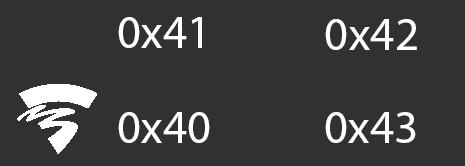
\includegraphics[width=\linewidth]{pcb-ina-0.png}
    		\caption{Bottom PCB}
    	\end{subfigure}
    \begin{subfigure}[b]{0.4\linewidth}
    		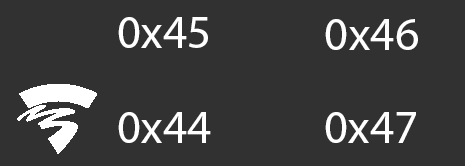
\includegraphics[width=\linewidth]{pcb-ina-1.png}
    		\caption{Top PCB}
    \end{subfigure}
    \caption{PCB INA connector layout, following page 18 of \url{http://www.ti.com/lit/ds/symlink/ina260.pdf}}
    \label{inapcb}
\end{figure}\newline
After that, make sure every Pi has it's own ethernet connection to the switch. If everything is setup correctly, it should work with the provided settings file "pis.xml" in the ina260 folder, the file will be required when starting the logger.\newline
\newline
\textbf{NOTE:}
\begin{itemize}
	\item In the current release of Debian Buster, the Pi picks only one of two interfaces (WiFi or Ethernet). Keep this in mind when trying to connect the Pi's to your hotspot.
\end{itemize}
Now you can make sure the Pi is authorized to access the HvA gitlab servers with an account.
\newline
The last step for setup, also the most essential for running, is to add all the Raspberry Pi's that you want to measure to your \code{/etc/hosts} file. For example, to add \code{raspberrypi-0}, you would write\newline
\code{0.0.0.0 raspberrypi-0.local}\newline
Where \code{0.0.0.0} has to be the actual IP address associated with the hostname. We have not been able to find out why this is necessary, but it seems that the logging programme is not able to do a reverse DNS lookup on it's own.
\subsection{Installation} \label{linstall}
To install the logger, make sure you have the data logger pi setup in your ansible hosts file. In our case this file was located in  \code{/etc/ansible/hosts} and contained the following lines:\newline 
 \code{[sgs]\newline
raspberrypi-g.local ansible\_user=pi}\newline
This means that you can run the playbook file \code{ansible/installG.yaml} with the following command: \code{ansible-playbook ansible/installG.yaml -l sgs}.
\subsection{Running}
To run the logger, you can now execute \code{powermonitoring/ina260/./ina260 -c pis.xml -d /home/pi/od}



\section{FFTW and MPI}

\subsection{Library's}
The test programs we use to simulate the load a astronomy supercomputer endures rely on a few library's. The FFTW\footnote{Fastest Fourier In The West} and the OpenMPI\footnote{Message Passing Interface} library. \par The FFTW library is used for the fourier transformations, it has integrated support for multi threading which is what one of the test programs uses. And it also has support for MPI which is what the other FFT test program uses. \par The MPI library is used for the communication between the pi's, and requires some know how to properly install. But if you follow this install guide everything should work. 

\subsection{Setup}
For the MPI programs to work it is important that all pi's can ssh to each other, since this is how they communicate. So they all need to be connected to the same network. In our setup two network switches are used to connect all the pi's to a router via ethernet cables, as shown on figure \ref{fig: Pi's with router}.
\begin{figure}[h!]
    \centering
    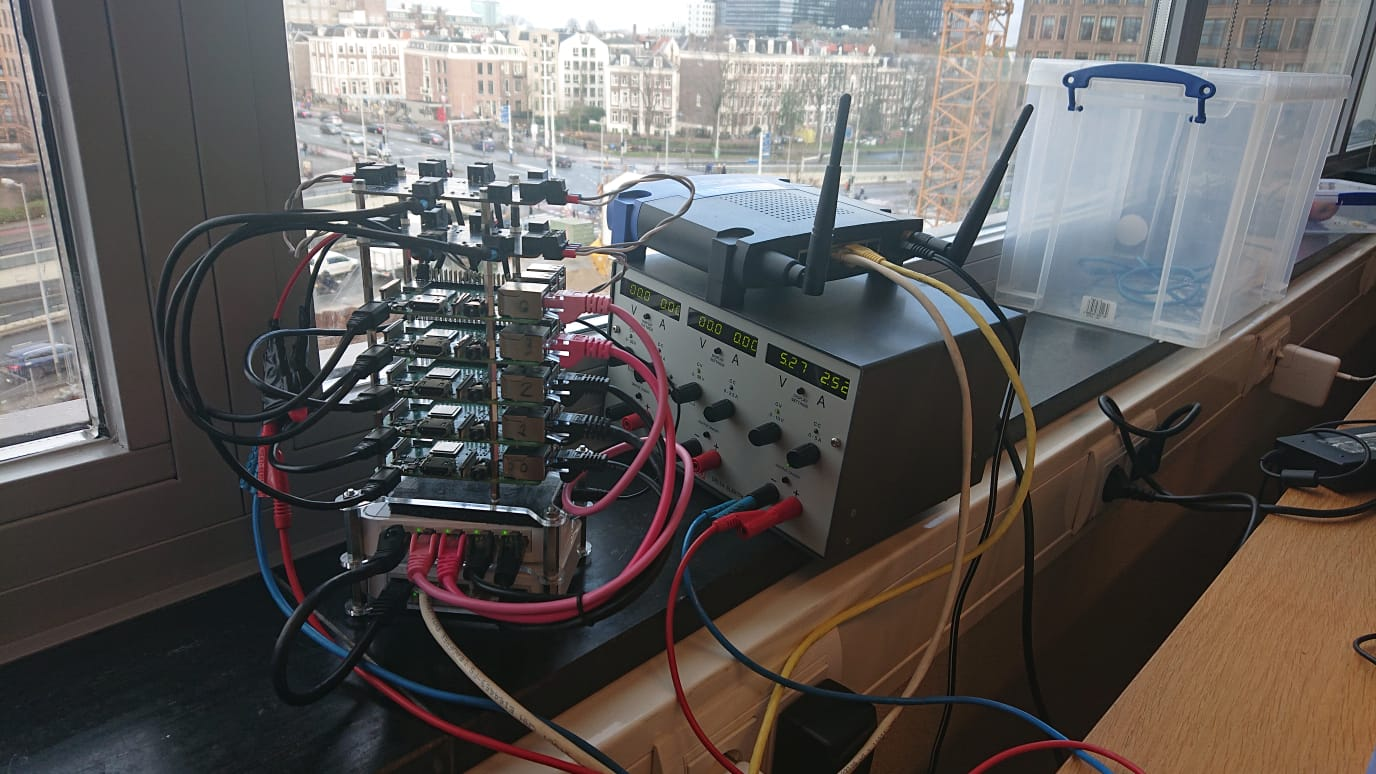
\includegraphics[width=\linewidth]{images/Pi_with_router.jpeg}
    \caption{Raspberryi pi's connected to router}
    \label{fig: Pi's with router}
\end{figure}

The process of giving each pi ssh access to each other has sadly not yet been automated and will have to be done manually. Each pi needs to have a ssh key and it's ID copy'd to all other pi's. To do this use the following commands:

\code{ssh-keygen}

followed up by,

\code{ssh-copy-id pi@[ip adress of each pi].local\\}


I've made a table you can use to keep track of which pi has ssh access to which other pi.
\begin{table}[h!]
\centering
\begin{tabular}{l|l|l|l|l|}
\cline{2-5}
                                          & pi-0 & pi-1 & pi-2 & pi-3 \\ \hline
\multicolumn{1}{|l|}{ssh-keygen}          &      &      &      &      \\ \hline
\multicolumn{1}{|l|}{ssh-copy-id to pi-0} &      &      &      &      \\ \hline
\multicolumn{1}{|l|}{ssh-copy-id to pi-1} &      &      &      &      \\ \hline
\multicolumn{1}{|l|}{ssh-copy-id to pi-2} &      &      &      &      \\ \hline
\multicolumn{1}{|l|}{ssh-copy-id to pi-3} &      &      &      &      \\ \hline
\end{tabular}
\end{table}

The ip adress of each pi is also needed for the machinefile, this is a file that MPI uses to know which "machines" it has avalible. 
A machinefile looks like this, Listing \ref{lst: machinefile}

\begin{lstlisting}[caption={Machinefile for MPI}\label{lst: machinefile}, frame=single]
pi@192.168.3.11 node0
pi@192.168.3.16 node1
pi@192.168.3.5  node2
pi@192.168.3.37 node3
\end{lstlisting}

And is located in the directory of the executable that uses MPI. (it can be located elsewhere but in the directory itself is easiest in my opinion) 

\subsection{Installation}

The install process has been automated using ansible scripts and is therefore very straightforward, we created a host group so the command can be sent to all pi's at once. 

To install the library's, make sure you have all the pi's that you want to run the programs on in your ansible hosts file. In our case this file was located in  \code{/etc/ansible/hosts} and contained the following lines:\newline 
 \code{[sfs]\newline
raspberrypi-0.local ansible\_user=pi\newline
raspberrypi-1.local ansible\_user=pi\newline
raspberrypi-2.local ansible\_user=pi\newline
raspberrypi-3.local ansible\_user=pi\newline
}

This means that you can run the playbook file \code{ansible/ansible\_install\_fftw.yaml} with the following command: 
\code{ansible-playbook ansible/ansible\_install\_fftw.yaml -l sfs}.

After this you can run the playbook \code{ansible/ansible\_install\_Test\_programs.yaml} with the following command: \newline \code{ansible-playbook ansible/ansible\_install\_Test\_programs.yaml -l sfs}.

\end{document}
